%!TEX root = cvl_bachelor_thesis.tex

%----------------------------------------------
% Introduction
%----------------------------------------------
\section{Introduction}
\label{sec:introduction}
Das Ziel dieser Projektarbeit war die Entwicklung eines webbasierten Frontends für eine Suchmaschine welche das Durchsuchen von radiologischen Bildern aus der Medizin ermöglicht.
Die Suchmaschine selbst ist ein Teil des KRESHMOI-Projekts \cite{kres} welches sich generell mit der Aufbereitung und dem Durchsuchen von medizinischen Informationen beschäftigt.
Das System KRESHMOI wird in diesem Kapitel erklärt und im speziellen wird auf die Suche für radiologische Bilder eingegangen.
Weiters werden die Anforderungen an das Frontend angeführt und auf die Möglichkeiten zur Umsetzung mit den am aktuellen Entwicklungsstand verfügbaren Technologien diskutiert.

%----------------------------------------------
% * Motivation 
%----------------------------------------------
\subsection{KRESHMOI}
\label{sec:Motivation}

Das Ziel von KHRESMOI ist das Durchsuchen und der Zugang zu medizinischen Informationen für verschiedene Benutzer-Gruppen mit unterschiedlichem medizinischen Vorwissen.
Die Einteilung der Benutzer erfolgt in 3 Kategorien:
\begin{itemize}
	\item Personen ohne speziellen medizinischen Kenntnissen
	\item Ärzte
	\item Radiologen
\end{itemize}
Dazu verknüpft KHRESMOI Daten aus verschiedenen heterogenen Ressourcen wie Bildern aus Radiologie-Archiven, Bildern und Text aus Publikationen in Journalen oder Daten von medizinisch relevanten Webseiten.
Da sich die verschiedenen Resourcen qualitativ sehr stark voneinander unterscheiden können wird ein Bewertung ihrer Glaubwürdigkeit durchgeführt und dem Benutzer angezeigt. 
%
Die Suchanfrage kann in textueller Form oder als Bild-Query sowie als Kombination von beidem gestellt werden.
Ein weiteres wichtiges Feature hierbei ist die multilinguale Suche, da die Menge an verfügbaren medizinischen Informationen nicht in alle Sprachen gleich ist.
Dies bedeutet dass die Suchanfrage in mehrere Sprachen übersetzt wird und somit auch anderssprachige Quellen durchsucht werden können.
Die Zusammenfassungen der Suchergebnisse werden anschließend in die Anfragesprache rückübersetzt, 
wodurch der Benutzer schnell durch die Ergebnissliste manchmal navigieren kann \cite{kres}.

Ein Teilprojekt von KHRESHMOI ist das Durchsuchen von medizinischen Bilddaten wobei diese in 2D oder 3D vorliegen können.
Um eine Suchanfrage auf ein Bild stellen zu können müssen an einem Ausgangsbild \C{eine oder mehrere sogenannte "Region(s) Of Interest" (ROI) eingezeichnet werden,} welche dann die Anfrage formen.
Aus der Textur eines markierten Bereiches wird ein Feature-Vektor extrahiert mit dem anschließend eine Datenbank von zuvor indizierten Bildern durchsucht wird.
%
Ein Frontend einer Bildsuchmaschiene muss daher sowohl Tools zum markieren von interessanten Bereichen, 
als auch die Funktionalität zur vernünftigen Betrachtung der Bilder bereitstellen \cite{kres}.

Diese Arbeit spezialisiert sich auf die Interaktion mit dem Teilsystem für das Durchsuchen von radiologischen Aufnahmen in 2D und 3D,
welche in einem PACS (Picture Archiving and Communication Systems) abgelegt sind.
Da in einem Krankenhaus täglich große Mengen an Daten durch radiologische Aufnahmen produziert werden, 
bietet eine effizientes Durchsuchen dieser die Möglichkeit  sie für Ausbildung und Forschung wieder zu verwenden.
%
Dazu muss das User-Interface die grundlegenden Funktionen eines Betrachtungstools für Röngten- und Computertomographie-Aufnahmen zur Verfügung Stellen:
\begin{itemize}
	\item Zoom
	\item Schnelles anpassen von Kontrast und Helligkeit
	\item Navigation durch die Schnitte eins 3D-Körpers (Volume) in einer Schnittachse
\end{itemize}
\cite{pacs}

%----------------------------------------------
% ** Java basiertes Interface
%----------------------------------------------
\subsubsection{Java basiertes Interface}
\label{sec:Java basiertes Interface}
Paralell zu dieser Applikation wurde im Rahmen des KRESMOI-Projektes auch einen auf Java basierendes Interface System entwickelt,
welches eine Schnittstelle zum vollständigen Funktionsumfang von KRESHMOI ist.
Bei diesem System gibt es verschiedene Versionen für Desktop, Browser, Mobile und eine spezielle Radiologie-Version \ref{fig:javabased_interface}, welche nur als Java Anwendung vorliegt.
Diese verfügt ebenfalls über Tools zum Betrachten und Interagieren mit den Volumes und zu erstellen von Bild-Suchanfragen.
Weitets bietes es Tools zum Durchsuchen von Fällen in einem Krankenhaus und weitere Features wie persönliche Bibliothek und kollaborative Tools.
Im gegensatz zur Java basierten Radiologie-Version liegt das Augenmerk bei diser Anwendung auf einen möglichst einfachen Zugriff und Verwendung durch den Browser.
\begin{figure}[t]
	\centering
	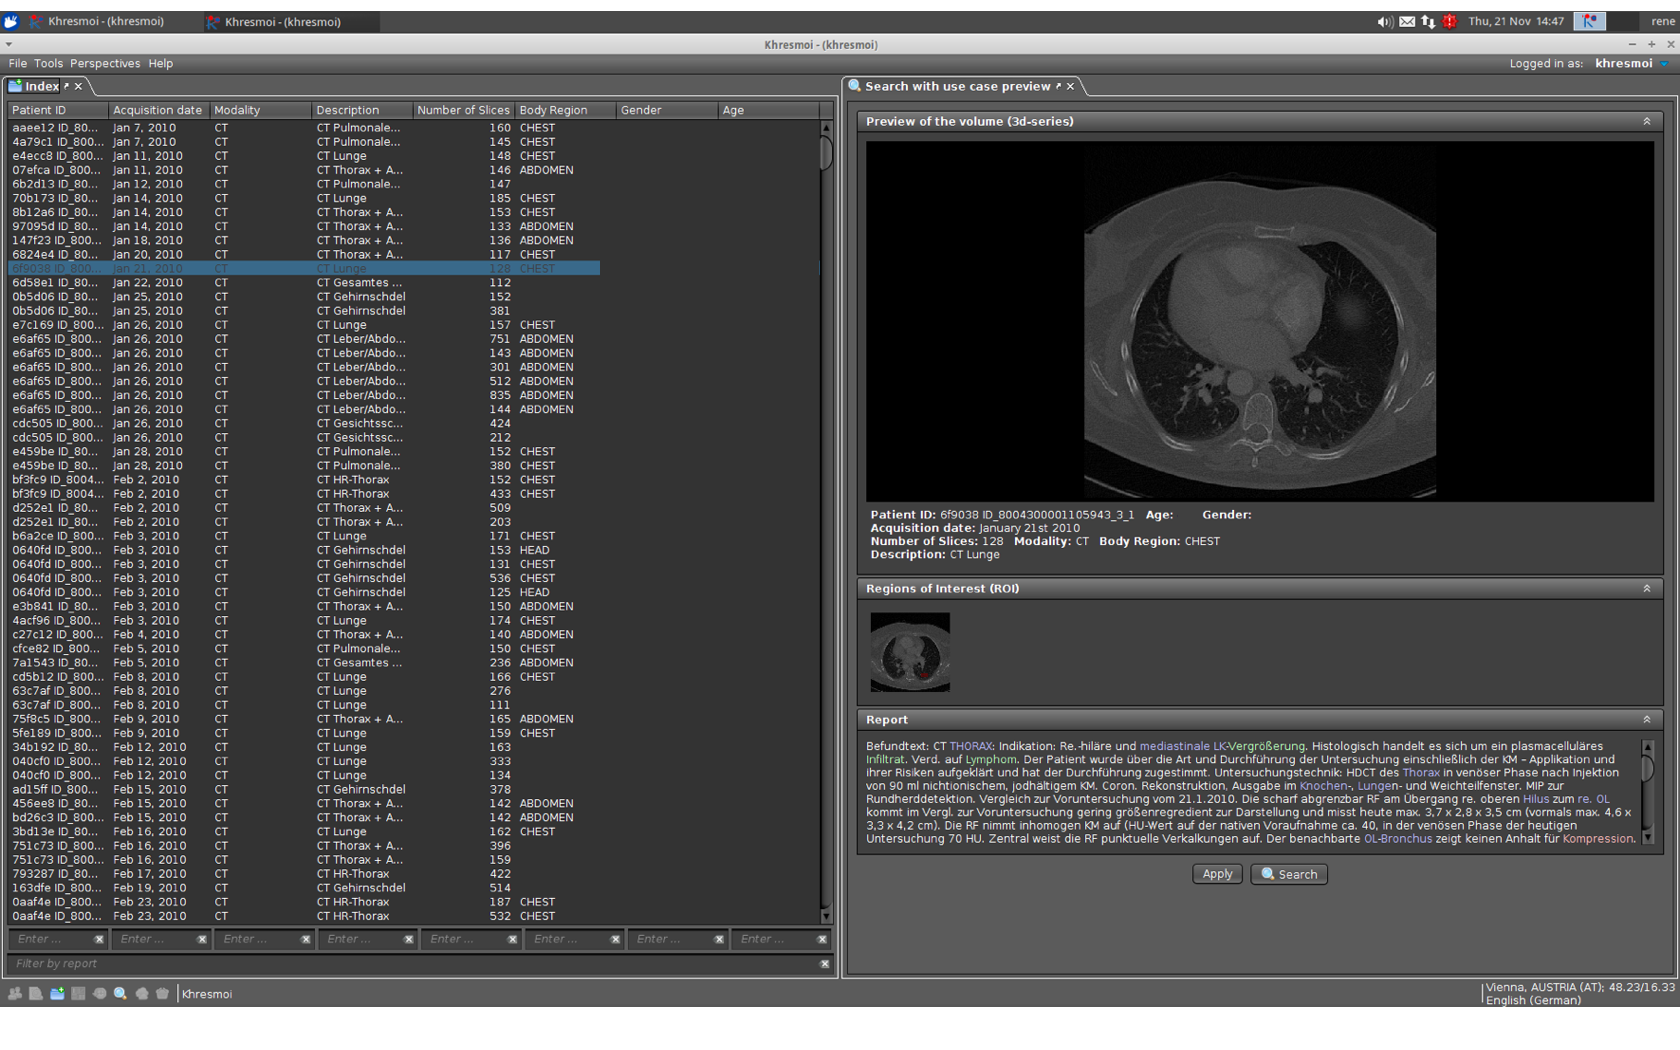
\includegraphics[width=0.8\linewidth]{img/c1_javainterface_indexview.png}
	\caption{Javabasierte Radiologie-Version des KRESHMOI Interfaces}
	\label{fig:javabased_interface}
\end{figure}

%----------------------------------------------
% * Pflichtenheft
%----------------------------------------------
\subsection{Pflichtenheft}
\label{sec:Pflichtenheft}
\begin{itemize}
	\item Kommunikation mit KRESHMOI über HTTP Anfragen. Dies beinhaltet das Senden von Suchanfragen, Auswerten der Ergebnisse und Laden der zugehörigen Bilder.
	\item Betrachten von CT Volumes. Navigation durch die einzelnen Schnitte eines Volumes entlang einer auswählbaren Achse.
	\item Schnelles anpassen von Kontrast und Helligkeit bei den einzelnen Schnittbildern mit der Maus (Fensterung).
	\item Zoomen und Scrollen des Bildausschnittes in einem Bild oder Volume.
	\item Tools zum Anotieren von Bereichen innerhalb der Bildern welche zur Interaktion mit der Bildsuche dienen.
	\item Präsentation der Suchergebnisse.
	\item Anzeige der den Bildern oder Volumes zugehörigen Reports.
	\item Ansicht zum Vergleichen von verschiedenen Ergebnissen.
	\item Modulare Komposition der verschiedenen Ansichten.
	\item Umsetzung der Applikation im Webbrowser.
\end{itemize}

%----------------------------------------------
% * Möglichkeiten zu Umsetzung
%----------------------------------------------
\subsection{Möglichkeiten zur Umsetzung}
\label{sec:Möglichkeiten zur Umsetzung}
Aufgrund der Anforderung, dass das Programm in einem Webbrowser ausgeführt werden soll, stehen derzeit drei Technologien zur Verfügung um die Anwendung umzusetzen.
Diese werden in den folgende Absätzen kurz angeführt und ihre Vor- und Nachteile im Bezug auf das Pflichtenheft untersucht.
Dabei spielt neben der Portabilität der Software, 
die Performance bei der Verarbeitung der Bilder einen große Rolle, da sowohl das Fenstern als auch das Navigieren durch die einzelnen Bilder einer 3D Aufnahme flüssig funktionieren müssen.

%----------------------------------------------
% ** JavaApplet
%----------------------------------------------
\subsubsection{JavaApplet}
\label{sec:JavaApplet}
Bei einem Java Applet \cite{japp} wird ein Java Programm in eine Webseite eingebunden und vom dem Browser des Clients geladen.
Der Browser übergibt das Applet dem Java Interpreter wofür aber ein spezielles Plugin notwendig ist. 
%
Der große Vorteil dieses Ansatzes ist dass die Anwendung sehr performant ist.
Dies ergibt aus den beiden Punkten dass Java Code compiliert wird und dass es möglichst ist die Grafikhardware des Clients zum Bearbeiten der Bilder zu verwenden,
welche für diese Aufgabe besser geeignet ist als die CPU.
%
Dafür müssen die notwendigen Plugins sowie ein aktueller Java Interpreter auf dem Client installiert sein, 
was bei manchen Betriebssystemen für Mobilgeräte wie Tablets gar nicht möglich ist \cite{japp}. 
\C{Als weiterer Nachteil gilt, dass JavaApplets ein nicht zu vernachlässigendes Sicherheitsrisiko darstellen,
obwohl prinzipiell nicht zertifiziert Applets durch eine Sandbox vom restlichen System isoliert werden.
Diese entstehen unter anderem durch Schwachstellen in der Sandbox, durch mangelnde Überprüfung der Zertifikate, 
zu schwache Sicherheitseinstellungen und durch Täuschung der Benutzer mit Testzertifikaten \cite{java_risks_cisico} \cite{java_risks_bmi}}.


%----------------------------------------------
% ** HTML5
%----------------------------------------------
\subsubsection{HTML5}
\label{sec:HTML5}
Bei diesem Ansatz wird die Anwendung in HTML, CSS und JavaScript oder einem Framework welches auf diesen Technologien aufsetzt entwickelt.
Die Entwicklung von Programmcode erfolgt bei Webapplikationen in JavaScript oder in Code für einen Interpreter welche in der JavaScript Laufzeitumgebung ausgeführt wird.
Da diese Technologien von fast allen neuen Browsern für Desktop und Mobilgeräte unterstützt werden, kann damit ein sehr hoher Grad an Portabilität erreicht werden.
Weiters sind Webapplikationen für den Benutzer sehr einfach zu verwenden da anstatt einer Installation um die Anwendung nutzen zu können nur eine Webseite geöffnet werden muss \cite{html}.

HTML5 \cite{html} unterstützt Canvas Elemente für 2D Bilder jedoch ist eine Verarbeitung der Bilder durch die Grafikhardware nur begrenzt möglich.
Für die Verwendung der Grafikarte durch den Browser gibt es die Schnittstelle WebGL \cite{webgl-14} welche auf OpenGL ES \cite{opengl-es-sepc} aufbaut.
Diese wurde jedoch noch nicht in allen gängigen Browsern implementiert oder ist in einigen noch nicht stabil und muss extra aktiviert werden \cite{webgl-14}.


%----------------------------------------------
% ** Flash 
%----------------------------------------------
\subsubsection{Flash}
\label{sec:Flash}
Flash Anwendungen sind Programme in einem proprietären Format das der Firma Adobe gehört.
Diese werden von einem Interpreter (dem Flash-Player) ausgeführt, welcher es über einen Browserplugin ermöglicht Flashcode in Webseiten einzubinden und mit der Webseite zu interagieren.
%
Die Erstellung von Anwendung erfolgt in der Entwicklungsumgebung Flash wobei Code in der objektorientieren Sprache Aktion-Script erstellt werden kann.
Flash bietet eine umfangreiche Grafik-API mit Unterstützung von Beschleunigung durch die Grafikkarte über OpenGL oder DirectX.
%
Die Darstellung von Flash-Inhalten im Browser setzt das Flash-Player-Plugin voraus.
Da es sich um ein proprietäres Format handelt ist der Support und die Weiterentwickung nicht sichergestellt \cite{flash-14}.
